%%
% Plantilla de reporte técnico para proyecto de listas enlazadas y sensores IoT
% Basado en plantilla IEEEtran
% Modificación: Diego Eduardo Zapata Aguilar - 30/OCT/2025
%
\documentclass[conference]{IEEEtran}

\usepackage[spanish]{babel}
\usepackage{amsmath,amssymb,amsfonts,amsthm}
\usepackage{graphicx}
\usepackage[utf8]{inputenc}
\usepackage{url}
\usepackage{hyperref}
\usepackage{subfig}
\usepackage{lipsum}
\usepackage{balance}
\usepackage{listings}
\usepackage{xcolor}

% Configuración de listings para código C++
\lstset{
    language=C++,
    basicstyle=\ttfamily\footnotesize,
    keywordstyle=\color{blue},
    commentstyle=\color{green!60!black},
    stringstyle=\color{red},
    numbers=left,
    numberstyle=\tiny\color{gray},
    breaklines=true,
    frame=single,
    showstringspaces=false
}

%%%%%%%%%%%%%%%%%%%%%%%%%%%%%%%%%%%%%%%%%%%%%
% PARCHE PARA ELIMINAR LA FECHA DEL DOCUMENTO
\usepackage{etoolbox}
\makeatletter
\patchcmd{\frontmatter@RRAP@format}{(}{}{}{}
\patchcmd{\frontmatter@RRAP@format}{)}{}{}{}
\makeatother	
%%%%%%%%%%%%%%%%%%%%%%%%%%%%%%%%%%%%%%%%%%%%%

\usepackage{datetime}
\newdateformat{specialdate}{\twodigit{\THEDAY}-\twodigit{\THEMONTH}-\THEYEAR}
\date{\specialdate\today}

\renewcommand\spanishtablename{Tabla}
\renewcommand\spanishfigurename{Figura}

\begin{document}

%%%%%%%%%%%%%%%%%%%%%%%%%%%%%%%%%%%%%%%%%%%%%
% Definitions
\newcommand{\breite}{1.0}
\newcommand{\RelacionFiguradoscolumnas}{0.9}
\newcommand{\RelacionFiguradoscolumnasPuntoCinco}{0.45}
%%%%%%%%%%%%%%%%%%%%%%%%%%%%%%%%%%%%%%%%%%%%%

% Title
\title{Sistema de Gestión Polimórfica de Sensores para IoT con Listas Enlazadas\\
\large Estructura de datos - Unidad 2}

% Author
\author{\IEEEauthorblockN{Diego Eduardo Zapata Aguilar}
	\IEEEauthorblockA{Ingeniería en Tecnologías de la Información\\
		Universidad Politécnica de Victoria\\
		Semestre: Sep-Dic 2025}
}

\maketitle

\begin{abstract}
Este proyecto presenta la implementación de un sistema de gestión polimórfica de sensores IoT utilizando estructuras de datos dinámicas (listas enlazadas simples) en C++. El sistema integra sensores de temperatura y presión con comunicación serial a través de Arduino, demostrando conceptos fundamentales de programación orientada a objetos como herencia, polimorfismo y gestión dinámica de memoria. Se implementaron contenedores genéricos mediante plantillas (templates) para el almacenamiento eficiente de lecturas, y se desarrolló una interfaz de usuario interactiva por consola. El proyecto incluye documentación técnica completa generada con Doxygen y organización modular del código fuente.
\end{abstract}

\section{Introducción}

El Internet de las Cosas (IoT) ha transformado la manera en que los dispositivos interactúan y recopilan datos del entorno. En este contexto, el desarrollo de sistemas capaces de gestionar múltiples tipos de sensores de forma eficiente y escalable es fundamental para aplicaciones de monitoreo en tiempo real.

Este proyecto aborda el diseño e implementación de un sistema de gestión de sensores que aprovecha las características de la programación orientada a objetos para crear una arquitectura flexible y extensible. El uso de listas enlazadas simples permite la gestión dinámica de sensores sin limitaciones de tamaño predefinido, mientras que el polimorfismo facilita el procesamiento uniforme de diferentes tipos de sensores.

\subsection{Objetivos}

\begin{itemize}
    \item Implementar estructuras de datos dinámicas (listas enlazadas simples) para gestión de sensores
    \item Aplicar conceptos de herencia y polimorfismo en un contexto práctico
    \item Desarrollar comunicación serial con Arduino para adquisición de datos
    \item Demostrar el uso de plantillas (templates) para código genérico y reutilizable
    \item Generar documentación técnica profesional mediante Doxygen
\end{itemize}

\section{Manual Técnico}

\subsection{Diseño del Sistema}

El sistema está diseñado siguiendo principios de programación orientada a objetos, con una arquitectura de tres capas:

\subsubsection{Capa de Abstracción de Sensores}

La clase base abstracta \texttt{SensorBase} define la interfaz común para todos los tipos de sensores:

\vspace{0.3cm}
\begin{lstlisting}
class SensorBase {
public:
    SensorBase(const char* nom);
    virtual ~SensorBase();
    virtual void procesarLectura() = 0;
    virtual void imprimirInfo() const = 0;
protected:
    char nombre[50];
};
\end{lstlisting}
\vspace{0.2cm}

Esta clase proporciona:
\begin{itemize}
    \item Métodos virtuales puros para garantizar implementación en clases derivadas
    \item Destructor virtual para correcta liberación de memoria polimórfica
    \item Encapsulamiento de datos comunes (nombre del sensor)
\end{itemize}

\subsubsection{Capa de Especialización}

Las clases concretas \texttt{SensorTemperatura} y \texttt{SensorPresion} heredan de \texttt{SensorBase} y especializan el comportamiento:

\begin{itemize}
    \item \textbf{SensorTemperatura}: Maneja lecturas tipo \texttt{float}, calcula promedios y elimina valores mínimos
    \item \textbf{SensorPresion}: Maneja lecturas tipo \texttt{int}, calcula estadísticas básicas
\end{itemize}

Cada sensor mantiene un historial de lecturas mediante la plantilla \texttt{ListaSensor<T>}.

\subsubsection{Capa de Gestión}

La clase \texttt{ListaGeneral} actúa como contenedor principal:

\vspace{0.3cm}
\begin{lstlisting}
class ListaGeneral {
private:
    Nodo<SensorBase*>* cabeza;
public:
    void insertar(SensorBase* valor);
    void procesarTodos();
    SensorBase* buscarPorNombre(const char* nombre);
};
\end{lstlisting}
\vspace{0.2cm}

Implementa operaciones de:
\begin{itemize}
    \item Inserción dinámica de sensores
    \item Recorrido polimórfico para procesamiento
    \item Búsqueda por identificador
    \item Liberación automática de memoria en cascada
\end{itemize}

\subsection{Componentes del Sistema}

\subsubsection{Estructuras de Datos}

\textbf{Nodo Genérico (\texttt{Nodo.h})}

Plantilla de nodo para listas enlazadas simples:

\vspace{0.3cm}
\begin{lstlisting}
template <typename T>
class Nodo {
public:
    Nodo<T>* siguiente;
    T valor;
    Nodo(T valor);
};
\end{lstlisting}
\vspace{0.3cm}

\textbf{Lista de Sensores (\texttt{ListaSensor.h})}

Implementación genérica con operaciones de:
\begin{itemize}
    \item Inserción al final: $O(n)$
    \item Búsqueda de mínimo: $O(n)$
    \item Eliminación de valor: $O(n)$
    \item Cálculo de promedio: $O(n)$
\end{itemize}

\subsubsection{Comunicación Serial}

\textbf{Clase ArduinoReader}

Gestiona la comunicación POSIX con Arduino mediante \texttt{termios.h}:

\begin{itemize}
    \item Configuración a 9600 baudios
    \item Lectura línea por línea no bloqueante
    \item Sincronización post-reset del Arduino
    \item Gestión automática de recursos (RAII)
\end{itemize}

Protocolo de comunicación:

\vspace{0.2cm}
\begin{verbatim}
FORMATO: SENSOR_ID,VALOR\n
EJEMPLO: T-001,25.3
         P-105,1015
\end{verbatim}
\vspace{0.3cm}

\subsubsection{Sketch de Arduino}

El firmware simula dos sensores con las siguientes características:

\begin{table}[h]
\centering
\caption{Especificaciones de sensores simulados}
\label{tab:sensores}
\begin{tabular}{|l|l|l|l|}
\hline
\textbf{ID} & \textbf{Tipo} & \textbf{Rango} & \textbf{Tipo Dato} \\ \hline
T-001 & Temperatura & 20.0-29.9°C & float \\ \hline
P-105 & Presión & 1000-1020 hPa & int \\ \hline
\end{tabular}
\end{table}

\subsection{Desarrollo}

\subsubsection{Herramientas Utilizadas}

\begin{itemize}
    \item \textbf{Compilador}: GCC 13.3.0 (C++11)
    \item \textbf{Sistema de Build}: CMake 3.28
    \item \textbf{IDE}: CLion / Visual Studio Code
    \item \textbf{Documentación}: Doxygen 1.9.8
    \item \textbf{Control de Versiones}: Git
    \item \textbf{Hardware}: Arduino Uno (ATmega328P)
\end{itemize}

\subsubsection{Estructura del Proyecto}

\vspace{0.2cm}
\begin{verbatim}
proyecto/
|-- include/         # Archivos de encabezado (.h)
|-- src/             # Implementaciones (.cpp)
|-- build/           # Ejecutables compilados
|-- arduino/         # Firmware Arduino
|-- docs/            # Documentacion Doxygen
+-- reporte_latex/   # Documentacion LaTeX
\end{verbatim}
\vspace{0.2cm}

\subsubsection{Proceso de Compilación}

\vspace{0.3cm}
\begin{lstlisting}[language=bash]
# Configurar con CMake
cmake .

# Compilar
make -j2

# Ejecutar
./build/ListasEnlazadasSimples
\end{lstlisting}
\vspace{0.2cm}

\subsubsection{Generación de Documentación}

\vspace{0.3cm}
\begin{lstlisting}[language=bash]
# Generar docs con Doxygen
doxygen DoxyFile

# Abrir documentacion
xdg-open docs/html/index.html
\end{lstlisting}
\vspace{0.2cm}

\section{Implementación y Resultados}

\subsection{Interfaz de Usuario}

El sistema presenta un menú interactivo por consola con las siguientes opciones:

\begin{enumerate}
    \item Crear Sensor de Temperatura (float)
    \item Crear Sensor de Presión (int)
    \item Registrar Lectura desde Arduino
    \item Ejecutar Procesamiento Polimórfico
    \item Cerrar Sistema (liberación de memoria)
    \item Registro Manual de Lectura
\end{enumerate}

% Figuras con capturas de pantalla del sistema
\begin{figure}[h]
    \centering
    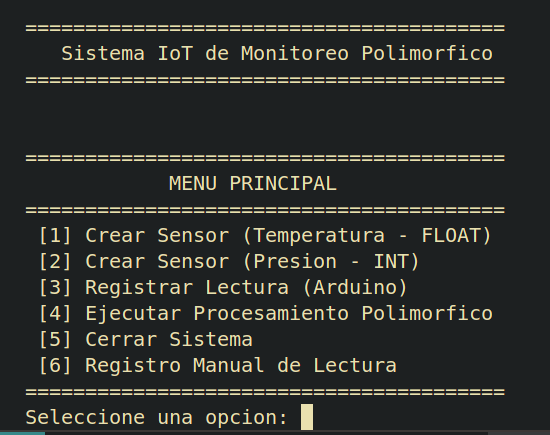
\includegraphics[width=\RelacionFiguradoscolumnas\columnwidth]{menu_principal.png}
    \caption{Menú principal del sistema de gestión de sensores}
    \label{fig:menu}
\end{figure}

\begin{figure}[h]
    \centering
    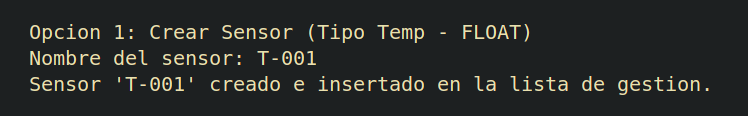
\includegraphics[width=\RelacionFiguradoscolumnas\columnwidth]{creacion_sensores.png}
    \caption{Proceso de creación de sensores de temperatura y presión}
    \label{fig:creacion}
\end{figure}

\begin{figure}[h]
    \centering
    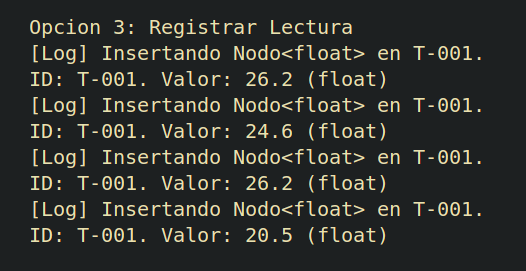
\includegraphics[width=\RelacionFiguradoscolumnas\columnwidth]{lectura_arduino.png}
    \caption{Adquisición de datos desde Arduino vía puerto serial}
    \label{fig:arduino}
\end{figure}

\begin{figure}[h]
    \centering
    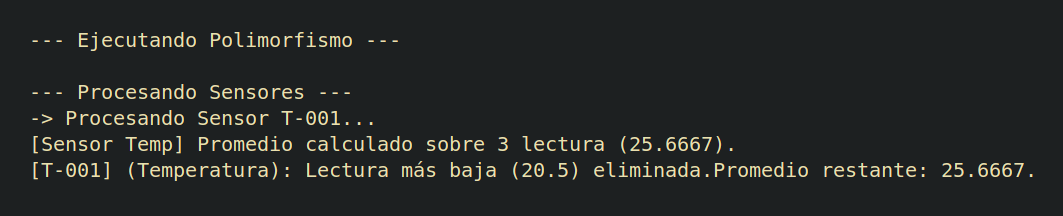
\includegraphics[width=\RelacionFiguradoscolumnas\columnwidth]{procesamiento_polimorfico.png}
    \caption{Ejecución del procesamiento polimórfico de sensores}
    \label{fig:procesamiento}
\end{figure}

\begin{figure}[h]
    \centering
    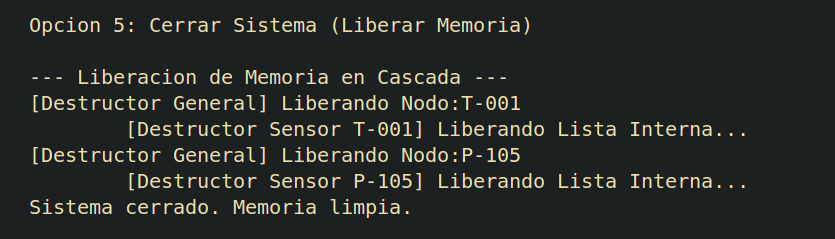
\includegraphics[width=\RelacionFiguradoscolumnas\columnwidth]{liberacion_memoria.png}
    \caption{Liberación de memoria en cascada al cerrar el sistema}
    \label{fig:destruccion}
\end{figure}

\subsection{Validación de Funcionalidad}

El sistema fue validado mediante:

\begin{itemize}
    \item \textbf{Pruebas de memoria}: Verificación con Valgrind (sin memory leaks)
    \item \textbf{Pruebas de comunicación}: Correcta recepción de datos desde Arduino
    \item \textbf{Pruebas de polimorfismo}: Procesamiento diferenciado por tipo de sensor
    \item \textbf{Pruebas de robustez}: Manejo de errores de conexión y datos inválidos
\end{itemize}

\subsection{Documentación Generada}

La documentación Doxygen incluye:

\begin{itemize}
    \item Jerarquía de clases con diagramas de herencia
    \item Documentación de cada método con parámetros y valores de retorno
    \item Ejemplos de uso y notas de implementación
    \item Índice alfabético de símbolos
    \item Código fuente navegable con resaltado de sintaxis
\end{itemize}

\section{Conclusiones}

Se logró implementar exitosamente un sistema de gestión polimórfica de sensores IoT que demuestra:

\begin{enumerate}
    \item \textbf{Estructuras dinámicas}: Las listas enlazadas permiten gestión flexible sin límites predefinidos
    \item \textbf{Polimorfismo}: El procesamiento uniforme de diferentes tipos de sensores mediante interfaces abstractas
    \item \textbf{Plantillas}: El código genérico reutilizable para diferentes tipos de datos
    \item \textbf{Comunicación serial}: Integración efectiva con hardware externo (Arduino)
    \item \textbf{Gestión de memoria}: RAII y destrucción en cascada garantizan ausencia de memory leaks
\end{enumerate}

El proyecto cumple con todos los objetivos planteados y constituye una base sólida para sistemas de monitoreo IoT más complejos. La arquitectura modular facilita la extensión con nuevos tipos de sensores y funcionalidades adicionales.

\subsection{Trabajo Futuro}

Posibles mejoras incluyen:
\begin{itemize}
    \item Implementación de persistencia de datos (archivos/base de datos)
    \item Interfaz gráfica con Qt o GTK+
    \item Soporte para múltiples Arduinos simultáneos
    \item Análisis estadístico avanzado de lecturas
    \item Alertas y umbrales configurables
\end{itemize}

\end{document}
